	\section{Requisitos}
		\subsection{Requisitos para la pestaña datos}
		\begin{enumerate}[\hspace*{0.5cm} %
			\bfseries Requ{i}s{i}to 1]
			\item Cada dato introducido en los campos de la pestaña \textbf{datos} debe ser validado y todos deben ser obligatorios llenarlos.
				\begin{enumerate}[a]
					\item Los campos; nombre, apellido paterno y apellido materno solamente permitirán el uso de letras, iniciando con mayúscula y las demás en minúsculas.
					\item El campo edad solamente permitirá números enteros.
					\item El campo fecha de nacimiento solamente aceptaran fechas en formado dd/mm/YY
					\item El campo CURP solamente aceptaran datos en formato de CURP.
					\item El campo usuario deberá contener una mayúscula, un numero y deberá ser mayor a 8 caracteres
					\item El campo contraseña deberá contener una mayúscula, un numero y deberá ser mayor a 8 caracteres
				\end{enumerate}
			\item Las demás pestañas estarán desactivadas hasta que la validación de la pestaña \textbf{datos} este completada.
			
		\end{enumerate}
		
		\subsection{Requisitos para la pestaña Licencia}
		\begin{enumerate}[\hspace*{0.5cm} %
			\bfseries Requ{i}s{i}to 1]
			\item Cada dato introducido en los campos de la pestaña \textbf{Licencia} debe ser validado y todos deben ser obligatorios llenarlos.
				\begin{enumerate}[a]
					\item El numero de control se generará incluyendo la fecha, es decir un código que asignen y se agregará a la cadena la fecha de 6 dígitos (requisito ambiguo).
					\item El campo tipo de licencia tendrá tres opciones: chófer, automovilista y motociclista.
					\item El campo fecha de registro la lee de sistema.
					\item El campo vigencia: 1, 3 o 5 años.
					\item El campo vencimiento se calcula en automático dependiendo de la vigencia.
					\item El campo observaciones sera de 200 caracteres, mostrar la cantidad de caracteres que faltan.
				\end{enumerate}
			\item La pestaña \textbf{captura de foto} estará desactivada hasta que la pestaña \textbf{Licencia} este completada.
		\end{enumerate}
		
		\subsection{Requisitos de la pestaña Captura de foto}
			\begin{enumerate}[\hspace*{0.5cm} %
			\bfseries Requ{i}s{i}to 1]
				\item En esta pestaña se mostraran los datos ya capturados.
				\item También se accederá a la cámara del computador para tomar la foto al solicitante y mostrarla junto con los datos
			\end{enumerate}
		\subsection{Requisitos del menú}
			\begin{figure}[h]
			\centering
				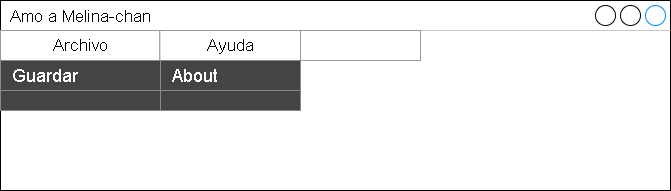
\includegraphics[height=3cm]{img/gui_menu}
				\caption{Boceto propuesto para el menú.}		
				\label{Pestaña menú}
			\end{figure}
			\begin{enumerate}[\hspace*{0.5cm} %
			\bfseries Requ{i}s{i}to 1]
				\item El primer menú sera \textbf{Archivo}, tendrá un submenú \textbf{Guardar}. Los datos se guardaran como objetos, no como archivo .txt. Usaremos la extención \textit{.melys} para el archivo de volcado de datos.
				\item El último menú será \textbf{Ayuda}, este tendrá un submenú \textbf{About}, dicho submenú lanzara un \textit{JFrame} donde se presentará la cara de Milina-chan con los datos de la aplicación, como: fecha de lanzamiento, version, autores, información de contacto y pagina web. 
			\end{enumerate}